\section{Results}
\begin{doublespacing}
\iffalse
In this study, heat conduction simulations were used to study the impact of overall heat transfer coefficient in the presence of Xenon bubble in the intragranular and intergranular region. Grain boundary resistance and the influence of intergranular fission is not included in this calculation. This simulation is design to see the impact on heat transfer due to the formation of Gas Bubble Superlattice. Bubble superlattice formation inside U-Mo fuel stabilizes the fuel swelling behavior but heavily impacts the heat transfer capability~\cite{burkes2015thermal}. This might be due to Xenon's very low thermal conductivity. Thermal properties of Xenon was also considered in this work. Xenon's thermal conductivity is a function of both temperature and pressure~\cite{rabinovich1987thermophysical}. Since the size of the bubble changes with the burnup and fission density, thermal conductivity of the bubble also changes~\cite{miller2012advantages}. Pressure inside the bubble is highly depend on the curvature of the bubble. The reults is plotted in figure~\ref{fig_result}. As it can be seen from the plot that thermal conductivity of U-10Mo drops with the presence of the Xenon bubble. And with the increase of the Xenon bubble's size it also decreases. The result is also compared with Maxwell-Eucken equation~\cite{maxwell1881treatise} and with Hashin and Strikman~\cite{hashin1962variational}. In figure~\ref{fig_compare} the comparison is showed. 
\fi

Figure~\ref{fig_result} shows the effective thermal conductivity due to Xenon bubble distribution in the intragranular region. Thermal conductivity decreases with the increase in the bubble size. In this simulation thermal conductivity of Xenon was at 1 bar. The FEM result is compared with the theoritical solution for porour material's thermal conductivity, to check whether the FEM results fall in the region. To compare the results the famous Maxwell-Eucken~\cite{maxwell1881treatise} equation was used. 
\begin{equation}
	\label{eq_MaxEuck}
	\lambda = \lambda_s\frac{\lambda_p+2\lambda_s+2\nu_p(\lambda_p-\lambda_s)}{\lambda_p+2\lambda_s-\nu_p(\lambda_p-\lambda_s)}
\end{equation}

\noindent Where, $\lambda = $ thermal conductivity of the fuel meat \\ 
		$\lambda_s = $ thermal conductivity of the continuous phase (U-10Mo) \\
		$\lambda_p = $ thermal conductivity of the dispersed phase in spherical shape (Xe bubble) \\
		$\nu_p = $ volume fraction of the dispersed phase (volume fraction of Xe inside U-10Mo) \\

Equation~\ref{eq_MaxEuck} assumes the pore volume fraction is less than 15$\%$ and dispersed uniformely in the solid matrix. The distance between the pores is far enough that they do not interact~\cite{clark2003monolithic,smith2013thermal}. The result is also compared with  Hashin-Shtrikman upper bound, which is based on a theoritical expression derived for the magnetic permeability of multiphase material~\cite{hashin1962variational}. 

\begin{equation}
\lambda = \frac{1}{4}\left [ \lambda_p(3\nu_p-1) + \lambda_s(2-3\nu_p) + \left \{ \left[ \lambda_p (3\nu_p -1) + \lambda_s(2-3\nu_p \right ]^2 + 8\lambda_s\lambda_p \right \}^\frac{1}{2} \right ]
\end{equation}



The compared result is shown in Figure~\ref{fig_compare}. As it can be seen from Figure~\ref{fig_compare} that with the increase in temperature there is a slight deviation.

\begin{figure}[H]
\centering
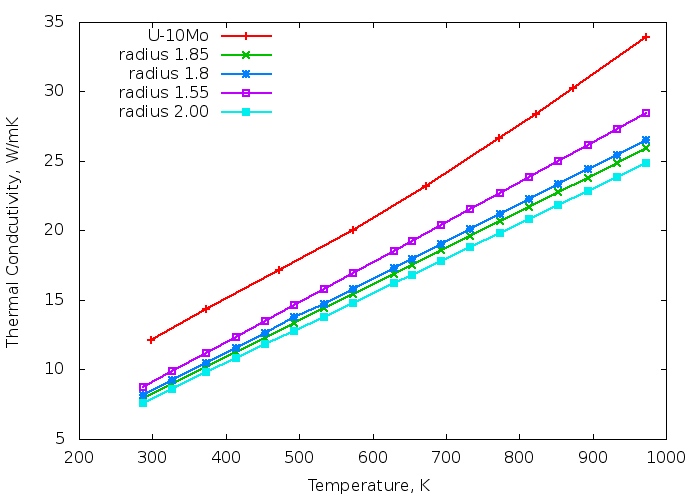
\includegraphics[scale=0.5]{result_Xe_U-10Mo.png}
\caption{Comparison between the thermal conductivity of U-10Mo and the inclusion of Xe bubble of different sizes}
\label{fig_result}
\end{figure}

\iffalse
FEM calculations were performed on \ref{fcc_mesh} in order to calculate the thermal flux and the thermal conductivity in 2D. Since thermal conductivity of Xenon is a function of both temperature and pressure, six different pressure has been chosen to represend the conductivity (Figure~\ref{fig_Xe_K}). Eventhough the dependence of thermal conductivity is evident, the results show no change in the overall thermal conductivity in the fuel. Pressure in the bubble is significantly higher than the 1000 bar in some situation~\cite{xiao2015atomistic}. The increased pressure inside the bubble creates another probability of having phase change from gas to solid~\cite{zheng2014thermodynamics}. The resluts show that with the increased pressure inside the Xenon bubble, the overall thermal conductivity has a very negligible effect. 
\fi

\begin{figure}[H]
	\centering
	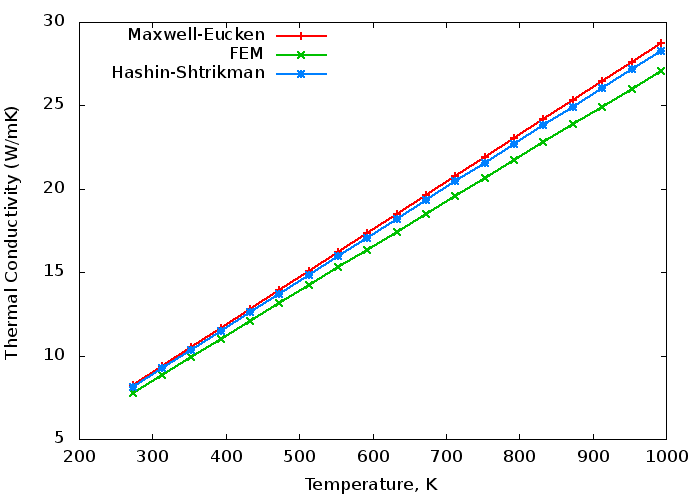
\includegraphics[scale=0.5]{theory_compare.png}
	\caption{Comparison of predicted thermal conductivity of U-10Mo with Xenon bubble against the Maxwell-Eucken and Hashin and Shtrikman }
	\label{fig_compare}
	\end{figure}
To see tha impact of pressure of Xenon on the overall thermal conductivity, five different pressures were used. Each pressure has a distinctvie thermal conductivity of Xenon(Figure~\ref{fig_Xe_K}). In this study a constant bubble size is used. The result of the simulations is presented in Figure~\ref{fig_press_K}. The result shows a little to no change on the overall thermal conductivity of the fuel meat. This might be due to the increasing pattern of thermal conductivity with respect to pressure.  

To study the grain boundary Xenon bubble, Xenon's thermal conductivity of 1 bar is used. The solution is obtained using Dirichlet boundary condition. The solution is presented in Figure~\ref{fig_eff_K_GB}. With addition of the grain boundary Xenon, overall thermal conductivity drops more than the addition of inragranular bubble.


\begin{figure}[H]
	\centering
	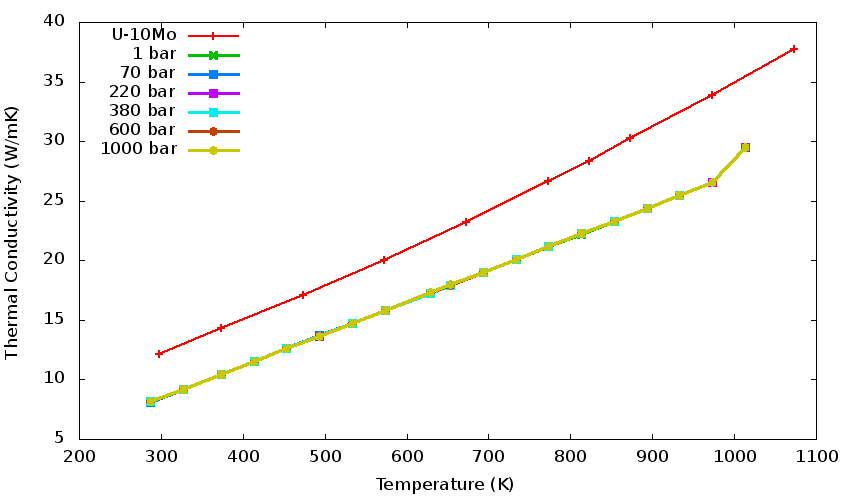
\includegraphics[scale=0.5]{press_eff_k.png}
	\caption{Over all thermal conductivity U-10Mo using thermal conductivity of Xenon of several pressure}
	\label{fig_press_K}
\end{figure}


\begin{figure}[H]
	\centering
	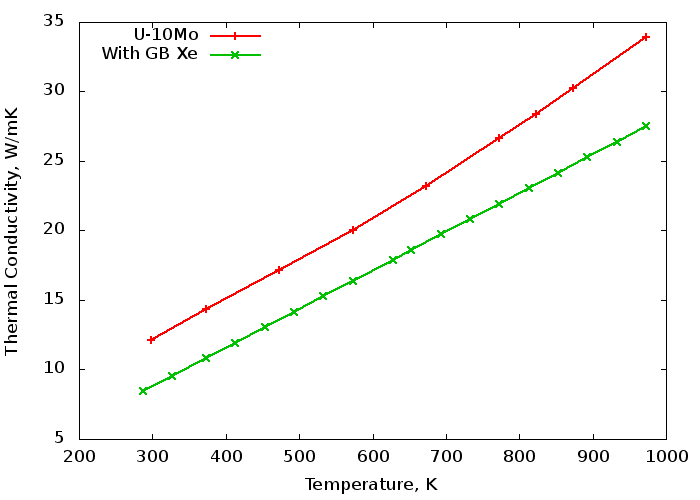
\includegraphics[scale=0.5]{result_Xe_GB.png}
	\caption{Over all thermal conductivity U-10Mo using grain boundary Xenon gas}
	\label{fig_eff_K_GB}
\end{figure}






\end{doublespacing}
